\documentclass[12pt,twocolumn]{article}



\usepackage{hyperref}
\usepackage{verbatim}
\usepackage[font=normalsize]{caption}
\usepackage{mathtools}
\usepackage{relsize}


\usepackage{amsmath}
\usepackage{graphicx}
\usepackage[capposition=bottom]{floatrow}
\usepackage{amssymb}
\usepackage{graphicx}
\usepackage{caption}
\usepackage{rotating}
\usepackage{afterpage}
\usepackage{float}
\usepackage{geometry}
\usepackage{titlesec}
\usepackage{epstopdf}

\usepackage{latexsym}
\usepackage{graphicx}
\usepackage{color}
\usepackage{array}
\usepackage{multirow}
\usepackage{wasysym}
\usepackage{verbatim}

\addtolength{\oddsidemargin}{-.875in}
\addtolength{\evensidemargin}{-.875in}
\addtolength{\textwidth}{1.75in}
%\addtolength{\voffset}{-70pt}
%\addtolength{\textheight} {120pt}

\hypersetup{
    bookmarks=true,         % show bookmarks bar?
    unicode=false,          % non-Latin characters in AcrobatÕs bookmarks
    pdftoolbar=true,        % show AcrobatÕs toolbar?
    pdfmenubar=true,        % show AcrobatÕs menu?
    pdffitwindow=false,     % window fit to page when opened
    pdfstartview={FitH},    % fits the width of the page to the window
    pdftitle={My title},    % title
    pdfauthor={Author},     % author
    pdfsubject={Subject},   % subject of the document
    pdfcreator={Creator},   % creator of the document
    pdfproducer={Producer}, % producer of the document
    pdfkeywords={keyword1} {key2} {key3}, % list of keywords
    pdfnewwindow=true,      % links in new window
    colorlinks=true,       % false: boxed links; true: colored links
    linkcolor=blue,          % color of internal links
    citecolor=green,        % color of links to bibliography
    filecolor=blue,      % color of file links
    urlcolor=cyan           % color of external links
}

\newcommand{\isot}[2]{$^{#2}$#1 }
\newcommand{\xeiso}{\isot{Xe}{136}}
\newcommand{\thsrc}{\isot{Th}{228}}
\newcommand{\cosrc}{\isot{Co}{60}}
\newcommand{\krsrc}{\isot{Kr}{83m}}
\newcommand{\cssrc}{\isot{Cs}{137}}
\newcommand{\nonubb}  {$0\nu \beta \beta$}

\renewcommand\thesection{\Roman{section}.}
\renewcommand\thesubsection{\arabic{subsection}.}
\renewcommand\thesubsubsection{\alph{subsubsection}.}
\titleformat{\section}[block]{\bfseries\filcenter}{\thesection}{1em}{}
\titleformat{\subsection}[block]{\bfseries\filcenter}{\thesubsection}{1em}{}
\titleformat{\subsubsection}{\bfseries\filcenter}{\thesubsubsection}{1em}{}

\usepackage{titlesec}

%\titleformat{\section}{\bfseries\filcenter}{\thesubsection}{1em}{}
%\titleformat{\subsection}{\bfseries\filcenter}{\thesubsection}{1em}{}
%\titleformat*{\paragraph}{\large\bfseries}
%\titleformat*{\subparagraph}{\large\bfseries}

\begin{document}

\title{Internal calibration of the LUX detector using tritiated methane}
\author{LUX Collab List}

\twocolumn[
\begin{@twocolumnfalse}
\maketitle

 \begin{abstract}

We present measurements of the electron-recoil (ER) response of the LUX dark matter detector using an internal tritium calibration source. The large-statistics tritium dataset provides ideal single-beta events with high purity and good spatial uniformity. We report on the charge and light yields of liquid xenon at 180 V/cm and 105 V/cm with high accuracy down to 1.3~keV energies, investigate fluctuations in the ER band, measure the energy threshold of the detector, and validate the combined energy model. These results provide input to the LUX Run3 WIMP search \cite{lux-reanalysis}.

\end{abstract}



\end{@twocolumnfalse}
]

\section{Introduction}

The Large Underground Xenon experiment (LUX) is a WIMP search located at the 4850' level of the Sanford Underground Research Facility (SURF) in Lead, South Dakota~\cite{lux-nim}. LUX detects particle interactions in liquid xenon (LXe) via scintillation (S1) and ionization charge (S2) signals. The LXe is instrumented as a dual-phase time projection chamber (TPC), providing an energy measurement, position information in three dimensions, and single-scatter event identification. Electron-recoil (ER) and nuclear-recoil (NR) events are distinguished by the ratio of the charge and light signals (S2/S1). Results from the first LUX science run (Run 3) were first reported in Ref.~\cite{lux-prl}. An improved analysis of the Run 3 data is reported in Ref.~\cite{lux-reanalysis}.

The LUX is monitored and calibrated primarily with electron sources that can be dissolved in the LXe. Two such sources,  \krsrc~\cite{Kastens:2009rt, Baudis} and tritium ($^{3}$H), have been deployed in LUX, both providing a large sample of spatially uniform events. In this article we report results from the calibration of LUX with tritium, a single-beta emitter with a Q value of 18.6~keV electron-equivalent\footnote{ER events and NR events generally have different energy scales in LXe. In this article we interpret all events using the ER energy scale.}~\cite{Tritium_Q}. 

The tritium beta spectrum is well known both theoretically and experimentally. It has a broad peak at 2.5~keV and a mean energy of 5.6~keV~\cite{Tritium_Mean,Tritium_Eq,Drexlin:2013lha}. 64.2\% of the decays occur between 1 and 8~keV, the energy range of interest for WIMP searches. These characteristics make it an ideal source for studying the ER response of LUX.  $\rm ^{83m}$Kr, which is a source of 9.4~keV and 32.1~keV internal conversion electrons, is well suited for routine monitoring and for correcting the spatial and temporal variations of the S1 and S2 signals, but is less useful for studies of the S2/S1 ER discrimination variable because both conversion electrons are above the dark matter energy range, and because the S2 signals from the two electrons generally overlap in the detector due to the short half-life of the intermediate state (154~ns). External gamma sources, such as \cssrc,  are also used on occasion by LUX, but they are unable to produce a useful rate of fiducial single-scatter calibration events in LUX in the WIMP energy range of interest due to self-shielding. We note that the most important background in LUX is due to Compton scatters, and such events are expected to have similar properties to beta decays in the tritium energy range. Neutron sources and a neutron generator are also employed by LUX to study the response to NR events~\cite{DD-paper}.

We use tritiated methane (CH$_3$T) as the host molecule to deliver tritium activity into LUX. Compared to molecular tritium (T$_2$), CH$_3$T has several advantages. It does not adsorb onto surfaces like the T$_2$ molecule, and it does not interfere with charge transport in LXe. Also, because of its 12.3 year half-life, tritium must be removed from the detector by purification, and methane is amenable to chemical removal with standard noble gas purifiers~\cite{Dobi_CH4}. Note, however, that diffusion of tritium activity into plastic detector components during the calibration is an important concern, since that activity may later re-contaminate the LXe during the WIMP search runs.  In this respect, CH$_3$T is preferable over T$_2$ due to its larger molecular size and lower diffusion constant and solubility~\cite{miyake:1983}. We investigated the CH$_3$T contamination risk empirically with a series of bench-top tests prior to the first injection into LUX. These tests, which are described in Appendix \ref{sec:appendix1}, demonstrated that the injection and removal could be done without undue risk to the experiment. 

An initial tritium dataset of $\sim$7,000 fiducial events was obtained by LUX in August of 2013, and the results were reported in Ref~\cite{lux-prl}. Subsequently, in December 2013, we injected additional activity with a higher rate and obtained a fiducial tritium dataset of 170,000 events. This dataset is used to characterize the LUX ER band in Ref.~\cite{lux-reanalysis}. Except where otherwise noted, in this article we report results from the larger December 2013 dataset.

\section{Development of the Calibration Source}

\subsection{Tritiated Methane Removal}
\label{sec:RD}

The removal efficiency of zirconium getters for methane in xenon had previously been studied at the University of Maryland.  It was found that greater than 99.99\% of natural methane can be removed in a single pass through a zirconium getter. \cite{Dobi_CH4} Tritiated methane is chemically identical to natural methane, so it follows that similar removal efficiencies should be expected for CH$_3$T.  To verify this a small scale tritiated methane injection system was integrated into a liquid xenon system at the University of Maryland.  This system used a SAES MC1-905F methane purifier placed in series immediately after the CH$_3$T source bottle to prevent non-methane species of tritium from entering the plumbing. Over 68,000 Bq of observed CH$_3$T activity was injected into this small scale system and a removal efficiency of over 99.99\% for tritiated methane in xenon was confirmed.

\begin{figure}[h!]\centering
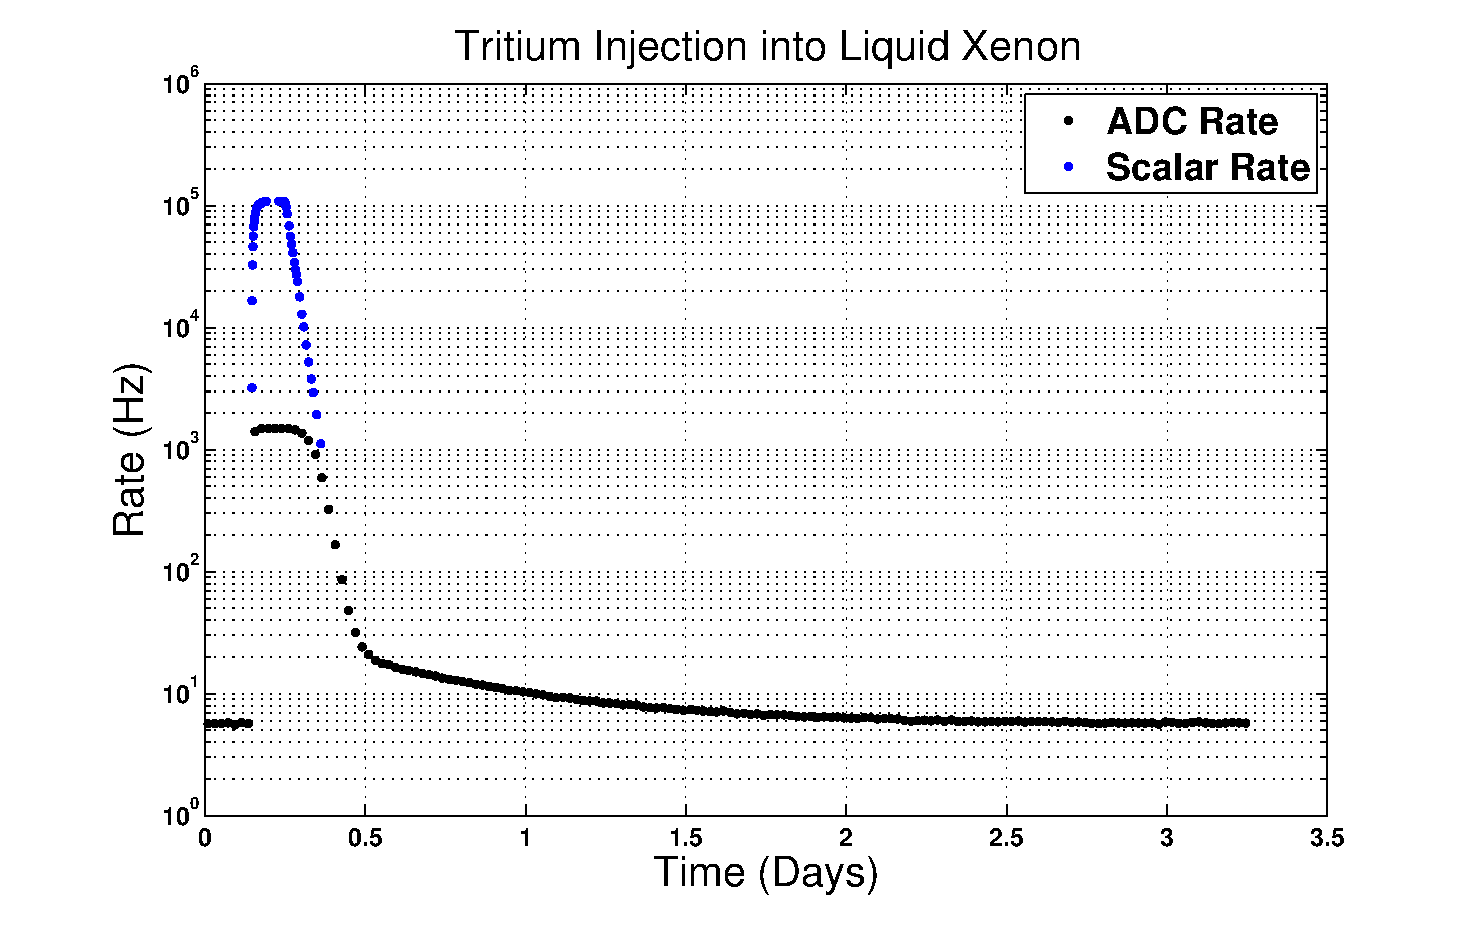
\includegraphics[width=80mm]{TimeHisto_Analog2.eps}
\caption{A time histogram of the event rate during a tritium injection into our small scale detector. The event rate greatly exceeded the limits of our ADC (black data points), so a analog scalar was used to count the true event rate (blue data points). }
\label{fig:Density}
\end{figure}


\subsection{Out Gassing of Tritiated Methane from Plastics}

\newcommand*{\Scale}[2][4]{\scalebox{#1}{$#2$}}%

An accurate model of a tritiated methane injection into LUX must account for out gassing of CH$_3$T from plastics such as polyethylene and teflon.  Using data from the liquid xenon experiments at the University of Maryland we numerically modeled the purification and residual diffusion of CH$_3$T in the detector.  Using Duhamel's priciple, the analytic solution to Fick's second law on a half-infite line is
\[\Scale[0.5]{\phi (x,t) = KC_{out} - \int \limits_0^t erf(\frac{x}{\sqrt{4D(t - \tau)}})K\dot{C_{out}}(\tau)d\tau - KC_{out}(0)erf(\frac{x}{\sqrt{4Dt}}),}\]
where $K$ is the solubility of the material, $D$ is the diffusion constant, and $C_{out}$ is the outside concentration of the material. \cite{Piche} For the out gassing process we are only able to detect the flux of material out of the plastic.  This is given by Fick's first law evaluated at $x=0$,
\[J_{out}(t)= - K \sqrt{\frac{D}{\pi}}( \int \limits_0^t \frac{\dot{C_{out}}(\tau)}{\sqrt{t-\tau}} d \tau + \frac{C_{out}(t)}{\sqrt{t}}),\]
where the sign has been flipped since the flux of material is outward.  We see that it is no longer possible to evaluate $K$ and $D$ separately, since the diffusion in and out of the plastic is completely determined by the time-dependent concentration outside of the plastic.  To simplify our model, we define a new constant
\[ G = K \sqrt{ \frac{D}{ \pi }} .\]
By fitting the integral of the flux out of the plastic over time to out gassing data collected in Maryland's liquid xenon system we constrain $G \leq 0.01 \; \frac{cm}{\sqrt{day}}.$ 

With a constraint on $G$ taken from the analytic solution to Fick's second law, we turn to numerical simulation to answer the question of how much initial CH$_3$T activity to inject into LUX to meet our calibration conditions.  Several assumptions are made to simplify the numerical model.  First, we approximate the diffusion into plastic as being a one dimensional process.  Since the plastic in our detector at Maryland and in LUX can be approximated by a cylindrical shell, there is no dependence on the azimuthal or $z$ coordinates.  Since $r$ is large compared to the thickness of the plastic shell, $\frac{\delta^2 \phi}{\delta r^2} \gg \frac{1}{r} \frac {\delta \phi}{\delta r}$, so Fick's laws in a one dimensional approximation become
\[J=-D\frac{\delta \phi}{\delta r}\vec{r}\]
\[\frac{\delta \phi}{\delta t} = D \frac{\delta^2 \phi}{\delta r^2}.\]  We assume the concentration of CH$_3$T in LUX is uniform throughout its volume, since the design of LUX creates currents which stir the liquid xenon.  With perfect mixing the effect of the purifier can be modeled by adding an exponential time dependence to the outer volume.  The time constant of this decay has an upper limit equal to the time it takes xenon to recirculate through the LUX detector, although in reality the mass transport from diffusion in the liquid and gaseous xenon decreases this time constant. 

We use a simple implementation of the first order Euler method for our numerical simulations. The diffusion is simulated by setting the concentration at the boundary of the piece equal to $KC_{out}$, where $C_{out}$ is the concentration of CH$_3$T in the xenon.  This concentration is dependent on time according to
\[\frac{\delta C_{out}}{\delta t} = J_{out} \frac{A_{plastic}}{V_{xenon}}-\frac{C_{out}}{\tau},\]
where $A_{plastic}$ is the surface area of the plastic cylinder, $V_{xenon}$ is the total volume of xenon in the fiducial region, and $\tau$ is the time it takes for one full purification cycle.  The first term on the right of this equation models out gassing of CH$_3$T from the plastic cylinder, while the second term models removal of CH$_3$T through purification.  Using the first order Euler method, we arrive at an expression for $C_{out}$ given by
\[C_{j+1}=C_j + \Delta t [(J_{1,j}-J_{N_x,j})\frac{A_{plastic}}{V_{xenon}}-\frac{C_j}{\tau}].\]
The initial concentration is defined by dividing the desired injection activity by the volume of the fiducial region.  We choose $D = 2.3 \times 10^{-9} \frac {cm^2}{sec}$ so that the half-infinite boundary conditions in our diffusion model is valid, and combine this with our allowed range of values for $G$ to extract a value for $K$.  We use this model to predict the total number of calibration events as well as the time required to return to \textless 5\% of the nominal background rate for any CH$_3$T injection into LUX.  

\begin{figure}[h]
\centering
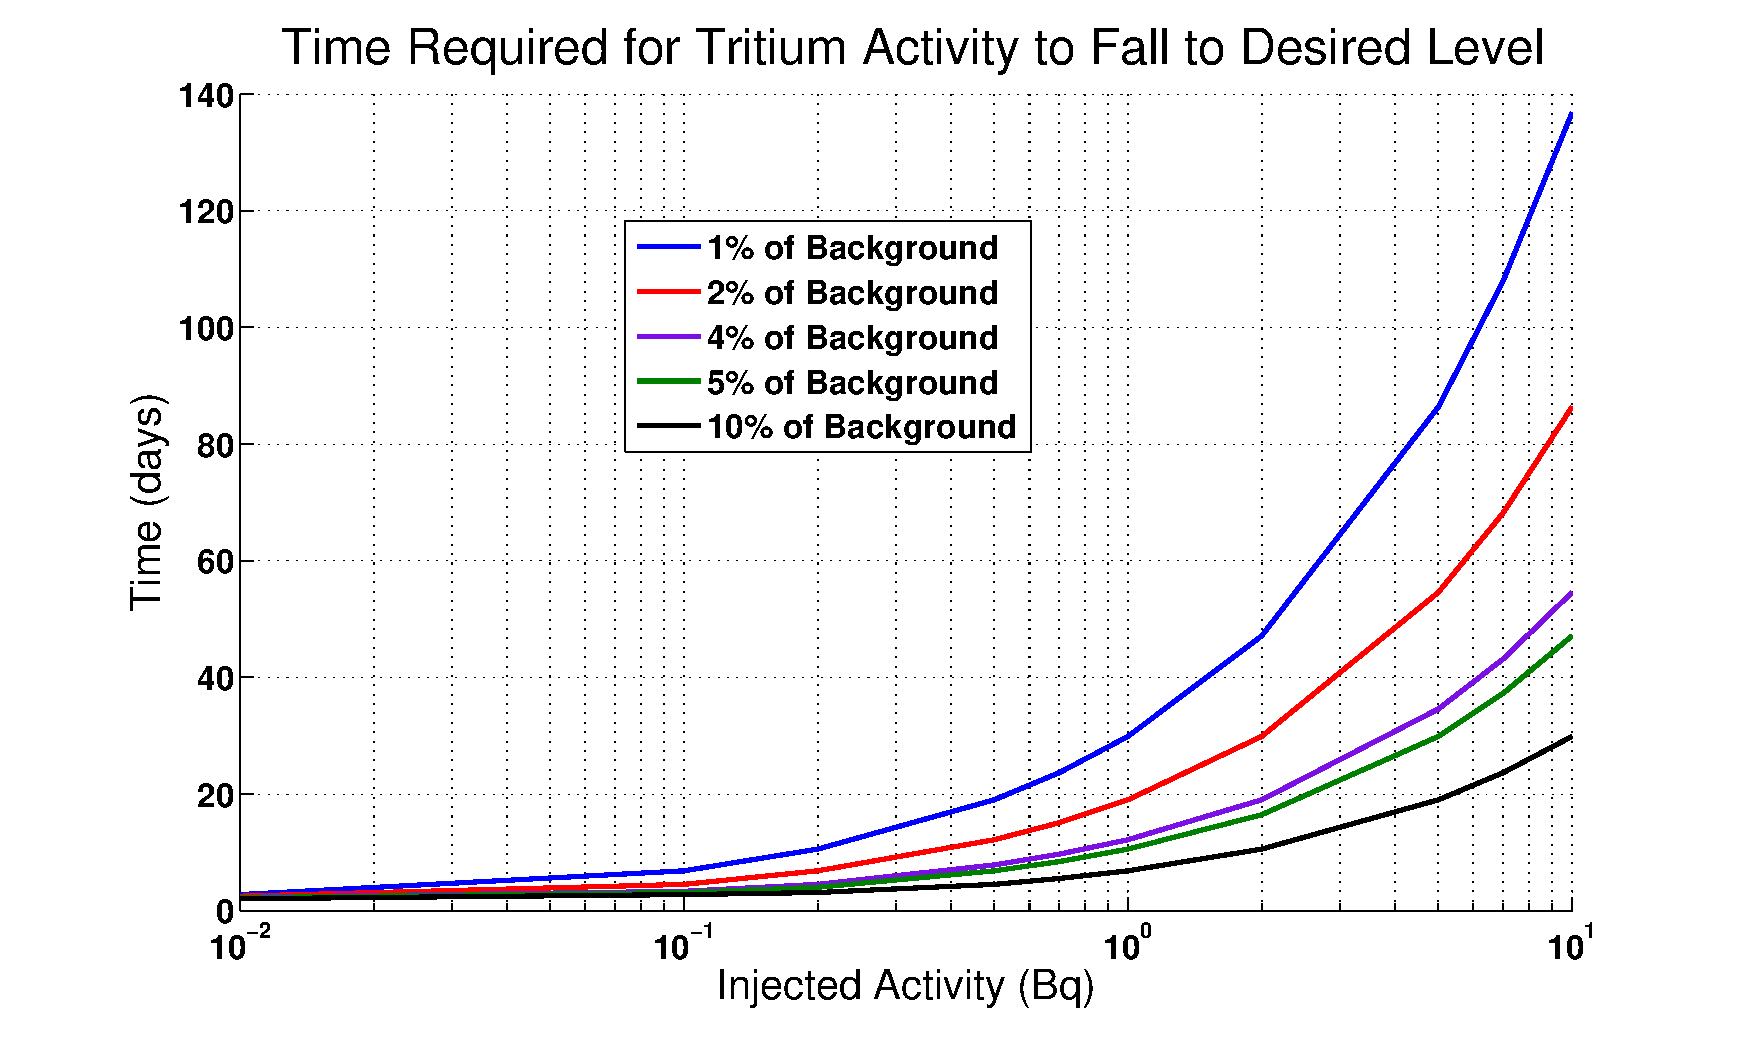
\includegraphics[scale=0.25]{LUXfig_INJvar_time_new.eps}
\caption{Time required to remove CH$_3$T from LUX after various injections.}
\label{fig:CH3TREMOVAL}
\end{figure}


\section{Implementation of the Calibration Source}

\subsection{Injection System Hardware}

The setup of our triated methane calibration technique can be separated into three parts: the tritiated methane source bottle, the injection system,  and the zirconium getter.

The tritiated methane source bottle for our calibration technique consists of a 2250 cc stainless steel bottle which is filled with a mixture of tritiated methane and purified xenon.  The purpose of this xenon is to serve as a carrier gas for the tritiated methane.  The total activity in the source bottle is set by mixing tritiated methane from a reservoir into the source bottle via volume sharing.

The injection system for our tritiated methane calibration technique consists of a series of expansion volumes which are used to fine tune the amount of CH$_3$T that is injected.  Once the CH$_3$T source bottle is opened it flows through a methane gas purifier (SAES MC1-905F) to remove any non-methane species of tritium, such as bare tritium. The expansion volumes are then filled with tritiated methane from the source bottle, and the flow of xenon in the gas system is diverted through the expansion volumes to sweep the CH$_3$T into the detector.  A pump out port allows the expansion volumes to be evacuated in preparation for each use of the injection system.  

The LUX gas system uses a hot zirconium getter (SAES-PS4MT15R1) located upstream of the CH$_3$T injection system to remove CH$_3$T from the xenon after passing through the detector.  

\begin{figure}[H]\centering
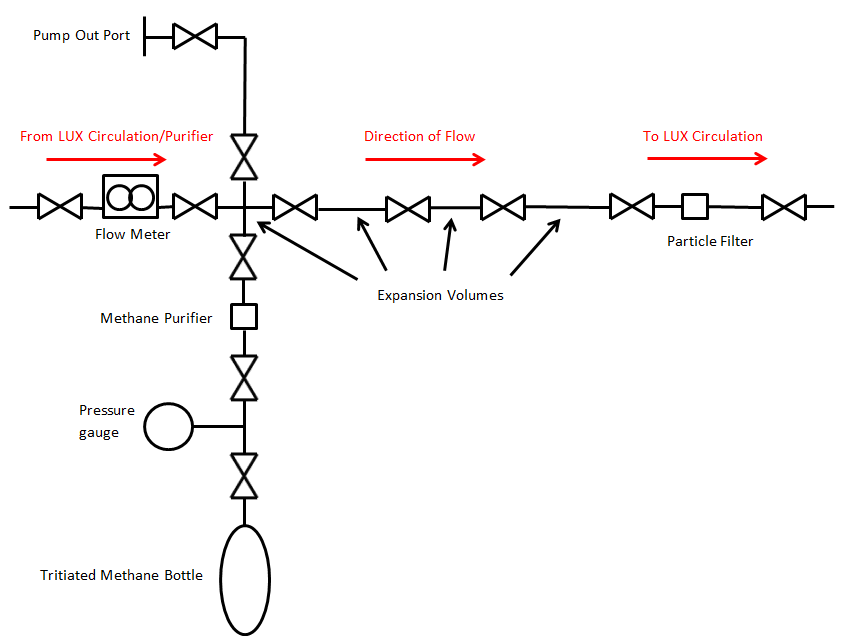
\includegraphics[width=80mm]{TritiumPlumbing.png}
\caption{Plumbing diagram of the tritium injection system for LUX.}
\label{fig:Removal}
\end{figure}

\subsection{Natural Methane Injection}

Prior to injecting tritiated methane into the LUX detector 0.02 grams of natural methane were injected into LUX using the injection system.  Purity samples from the detector were collected over the next few days, and a purification time constant of 5.90 $\pm$ 0.07 hours was determined using data collected with the LUX gas sampling system.



\begin{figure}[h!]\centering
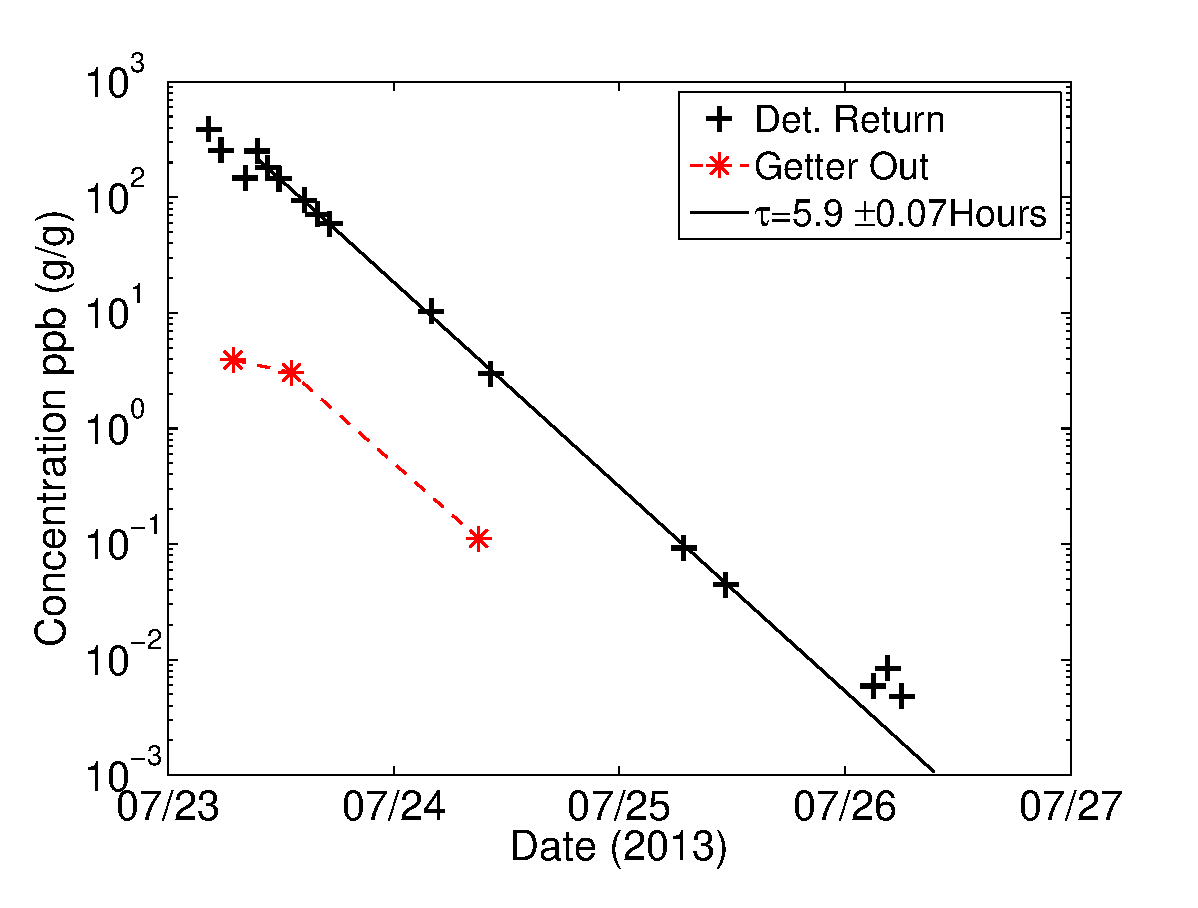
\includegraphics[width=80mm]{CH4_injection_3.eps}
\caption{Removal of natural methane observed by the integrated xenon sampling system prior to the tritiated methane injections. The red points indicate xenon gas measurements at the getter outlet, we find a 97\% one pass removal efficiency at a flow rate of 25 SLPM. 1 $\rm 10^{-3}$ ppb (g/g) is the limit of detection for methane using the LUX gas sampling system.}
\label{fig:Removal_methane}
\end{figure}


\subsection{Tritiated Methane Injection}

To confirm the purification model established by the natural methane injection a small amount of tritiated methane was injected into LUX the following week. An absolute activity of 20 mBq of tritiated methane was injected with the getter in purify mode.  Thus as soon as the CH3T passed through the detector it was immediately removed.  A purification time constant of 6.7 hours was observed, consistent with the natural methane purification rate measured by the sampling system. After a day of circulating through the getter the tritium decay had fallen below detectable amounts confirming the effective removal of the tritiated methane with the getter. 

After confirming our purification model a larger injection of 800 mBq was performed. This second injection produced 20,000 beta decay events in the LUX detector before being completely removed, 5000 of those events could be used the calibrate the ER band in the WIMP search region of 0-30 Phe (pulse area in photo electrons). 
Figure \ref{fig:Removal} shows the two tritium injections and the subsequent CH3T purification. The rate of tritiated methane removal was consistent with the previous two injections $\rm 1/10^5$.



\section{Results from the Tritiated Methane Calibration}



\subsection{Mixing of Tritiated Methane in Liquid Xenon}

Tritium events appear uniformly distributed in the liquid volume several minutes after injecting the tritiated methane inline with the xenon gas circulation path. Figure \ref{fig:Density} shows the XY and Z distribution of tritium events thirty minutes after an injection. The events shown cover the region from the gate to the cathode and radially out to the edge of the detector. An additional cut requiring that the event be between $\rm \pm 3 \sigma$ of the ER mean was made to diregard residual alpha events from the walls and cathode, the event rate consisted overwhelmingly of tritium events. The tritiated methane dispersed uniformly throughout the liquid xenon illuminating all regions on the detector. 
 
\begin{figure}[h!]\centering
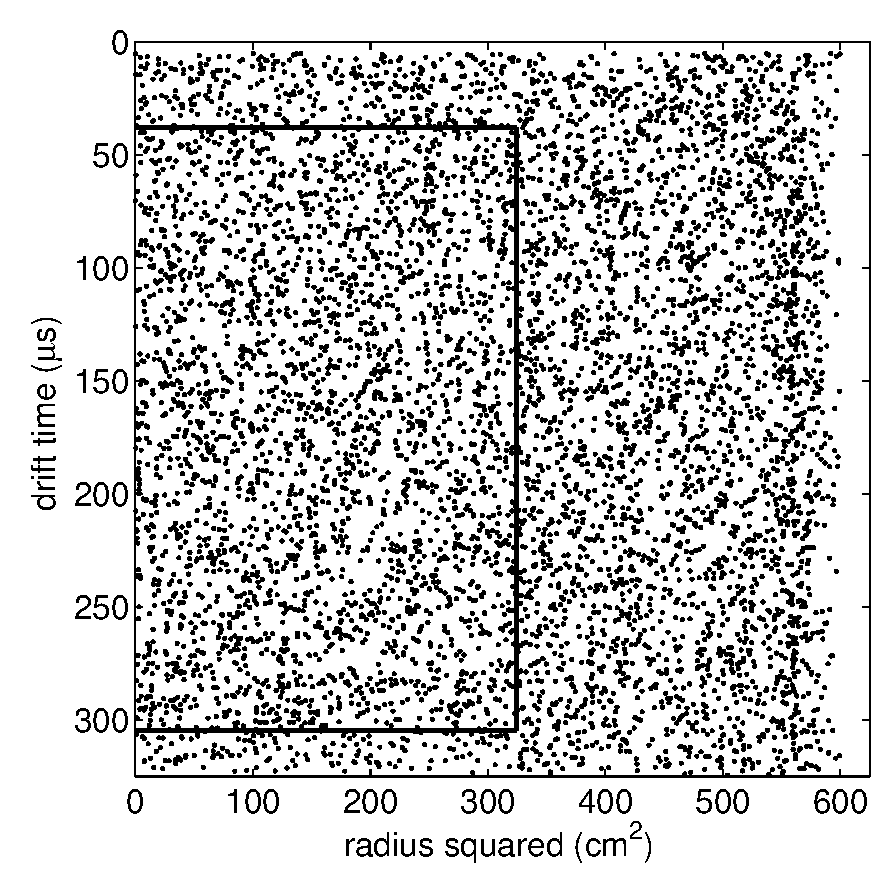
\includegraphics[width=80mm]{CH3T_RZ_scatter_lux10_20130812T1546.eps}
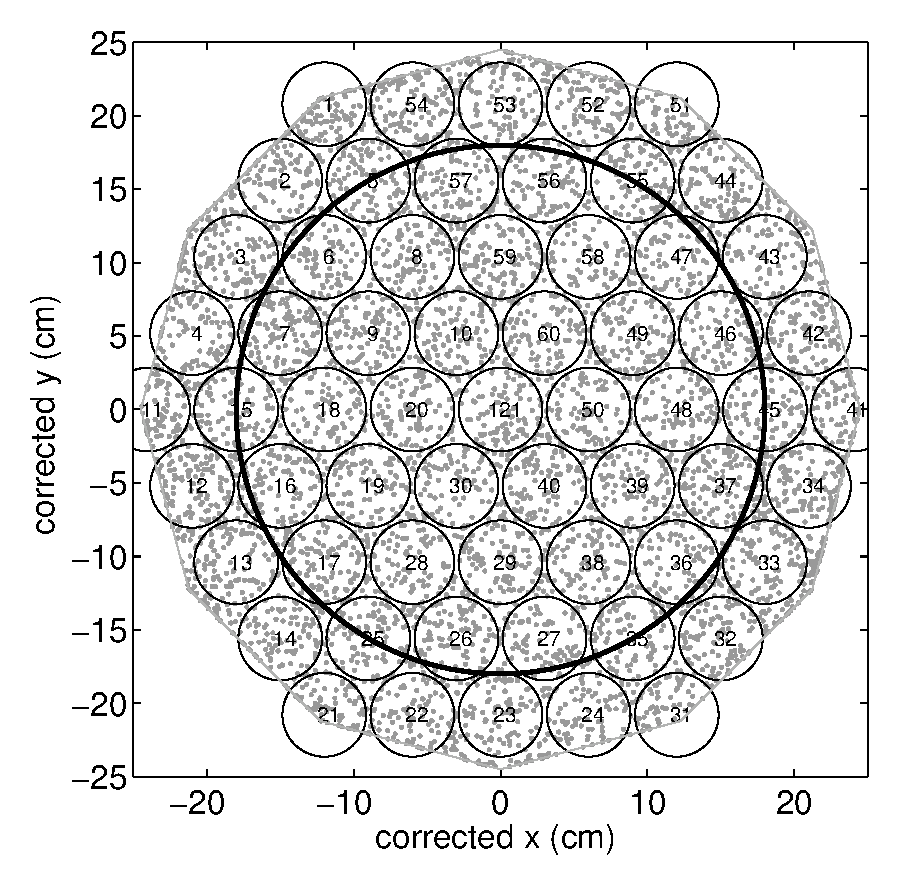
\includegraphics[width=80mm]{CH3T_XY_scatter_PMT_lux10_20130812T1546.eps}
%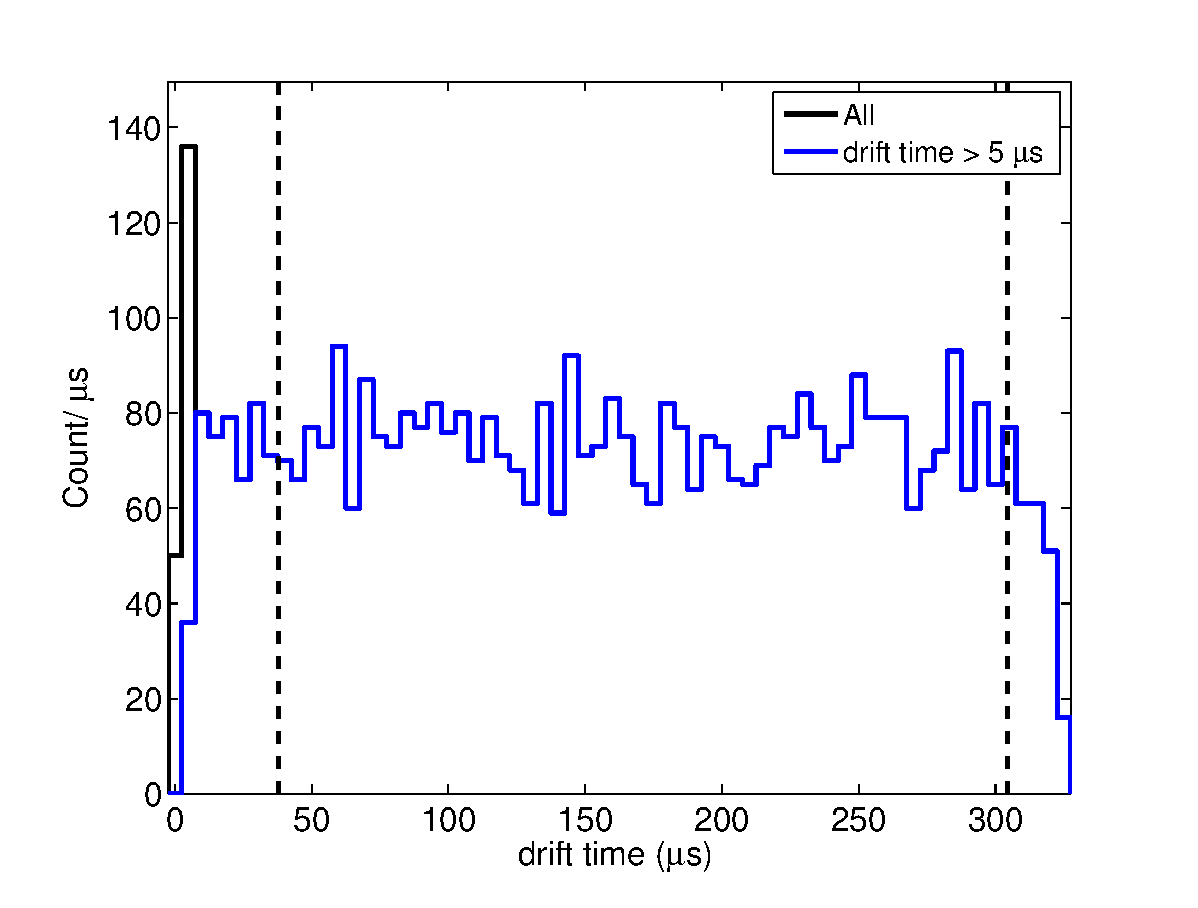
\includegraphics[width=80mm]{CH3T_Z_density_lux10_20130812T1546.eps} %> No Need R^2 vs. Z figure contains Z information
\caption{Left: The distribution of tritium events vs. detector radius squared. The solid black line represents the fiducial volume. Right: The distribution of tritium events vs. XY in the region between the gate and the cathode. The solid black line represents the fiducial volume and the black circles represent the locations of PMTs (photo multiplier tubes).}
\label{fig:Density}
\end{figure}




  \begin{comment}
... Remove this graphic, for smaller tritium injection
\begin{figure}[h!]\centering
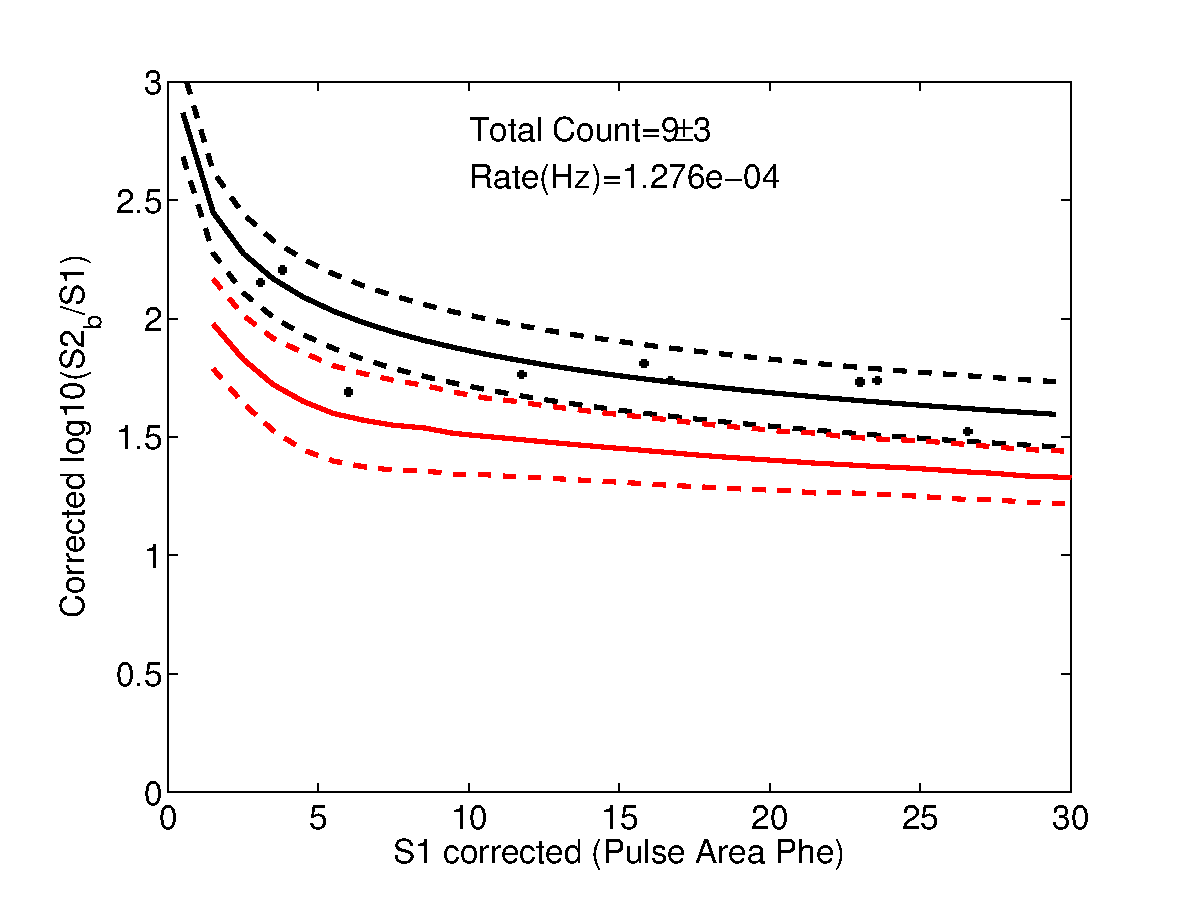
\includegraphics[width=80mm]{CH3T_fid_30_before_100_18_lux10_20130813T1120_cp05328_note.eps}
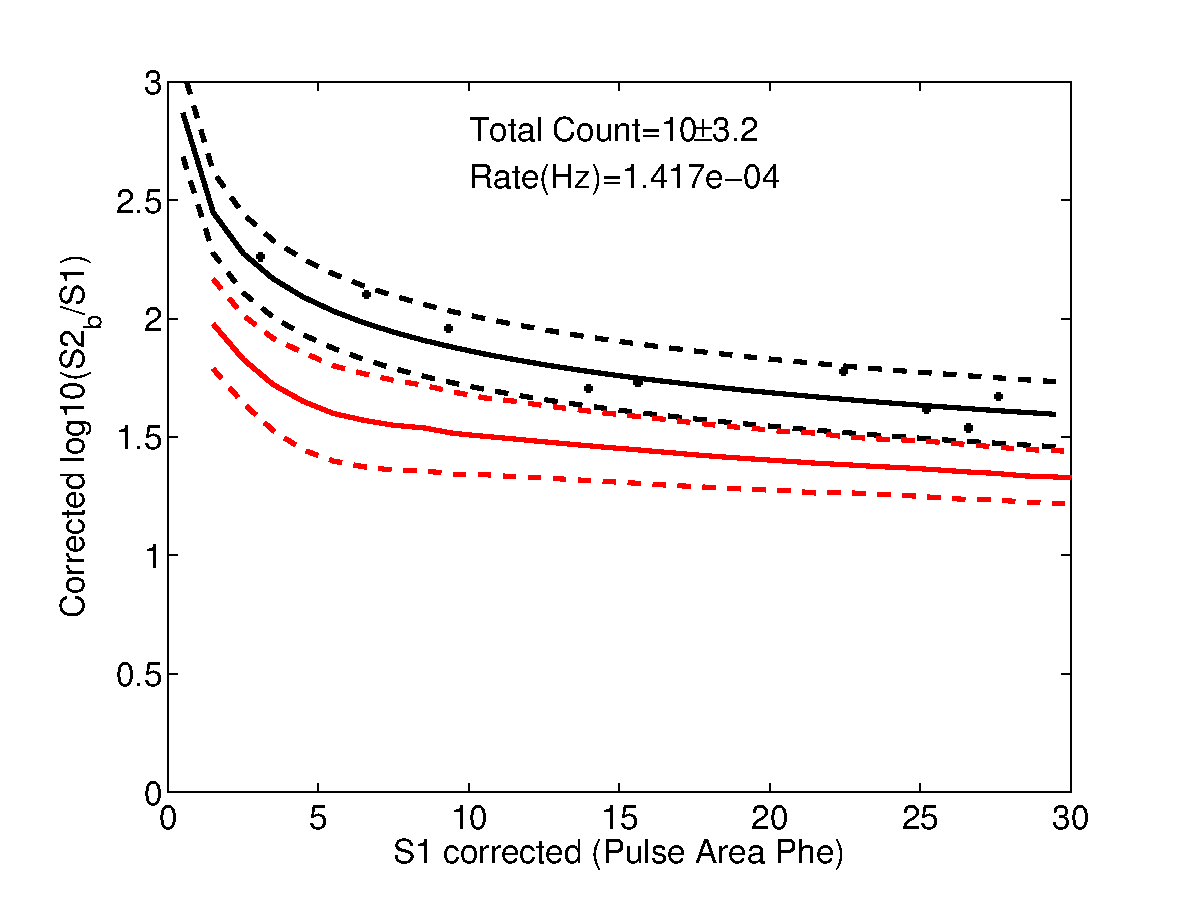
\includegraphics[width=80mm]{CH3T_fid_30_after_100_18_afterlux10_20130813T1120_cp05328_note.eps}
\caption{Left: 100 Hour time window in the WIMP search region before the tritiated methane injection. Right: 100 Hour time window in the WIMP search region after the purification of the tritiated methane. }
\label{fig:Removal_2}
\end{figure}

  \end{comment}

\subsection{Definition of Electronic Recoil Band and Comparison with NEST Model}

Using the tritium source we calibrated the electronic recoil band in the fiducial volume of the LUX detector to unprecedented accuracy. Figure \ref{fig:Band} shows the mean of the ER band along with the 10-90\% confidence bounds ($\pm 1.28\sigma$) obtained from the beta decay of tritium at a drift field of 180 V/cm. The results of the leakage fraction at 50\% NR acceptance per each 1 Phe bins in S1 are shown in \ref{fig:Leak}. The nuclear recoil band, in red, is defined by the NEST model along with AmBe and $\rm^{252}Cf$  calibrations. Methane will not quench xenon scintillation [\cite{Kirill_Methane}] shows that if methane is introduced into the xenon at a relative concentration of a few percent, then the amount of scintillation produced by the mixture is reduced by a factor of two compared to pure xenon. But for our application we require a methane concentration of only one part in $\rm10^{15}$, and therefore our methane injection will not have any negative effects on scintillation production and transport.

WIMPs primarily interact with the atomic nuclei xenon atoms in LUX resulting in nuclear recoils whereas the vast majority of residual radioactivity within the detector are gammas which result in electronic recoils. Thus, knowing the separation of the ER from the NR band allows for a measure of the background rejection of a liquid xenon WIMP search experiment. We define the measure of background rejection as leakage fraction, reported here as the fraction of events in the ER band that spill into the lower half of the NR band. Over 115,000 tritium decays were used for the ER band calibration, between 1-50 Phe in S1 (1-8 $\rm keV_{ee}$), and were found using standard WIMP search cuts within the fiducial volume. A figure of merit for ER and NR discrimination is the leakage fraction defined as  the number of tritium events populating the lower half of the NR band are compared to the total number of tritium events in the selected energy range. 
%$\rm (1-erf((Mean\_ER-Mean\_NR)/(sqrt(2)*sigma\_ER)))/2 $.
Figure \ref{fig:Leak} shows the leakage fraction per 1 Phe bins in S1. The mean leakage fraction in the region used for the LUX 2013 PRL results, between 1-30 Phe (1-5 $\rm keV_{ee}$) in the fiducial, was found to be 0.42\% $\rm \pm$ 0.02\%, see Figure \ref{fig:Leak}. In the 40 hour time window in which the data was acquired less than three out of 115,000 events are expected to be non tritium [BG paper reference]. The NR band used is from NEST version 0.98 and is vetted with AmBe, $\rm^{252}Cf$ and DD neutron generator calibrations.


\begin{figure}[h!]\centering
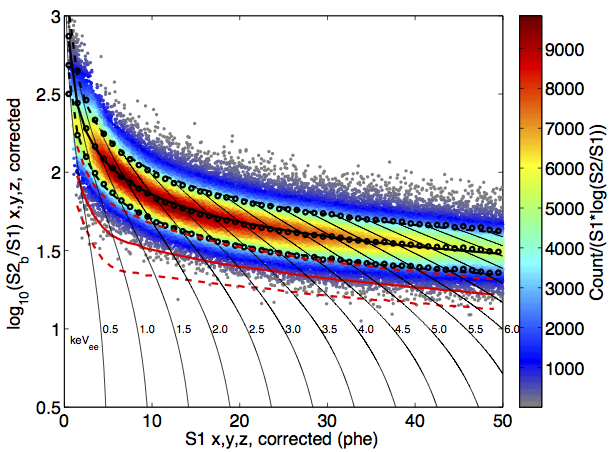
\includegraphics[width=80mm]{CH3T_fid_50_2_Dec_Tritium_Approval_Plots.png}
\caption{Discrimination vs. S1 using over 115,000 tritium beta decays between 1 and 50 Phe in S1 (about $\rm1-8 keV_{ee}$). On average from 1 to 30 Phe the discrimination is 99.58\%, defined by the fraction of events of events below the mean of the nuclear recoil band. The red band represents the NEST nuclear recoil band (version 0.98) vetted with an AmBe, $\rm^{252}Cf$ and DD neutron generator calibration.}
\label{fig:Band}
\end{figure}

\begin{figure}[h!]\centering
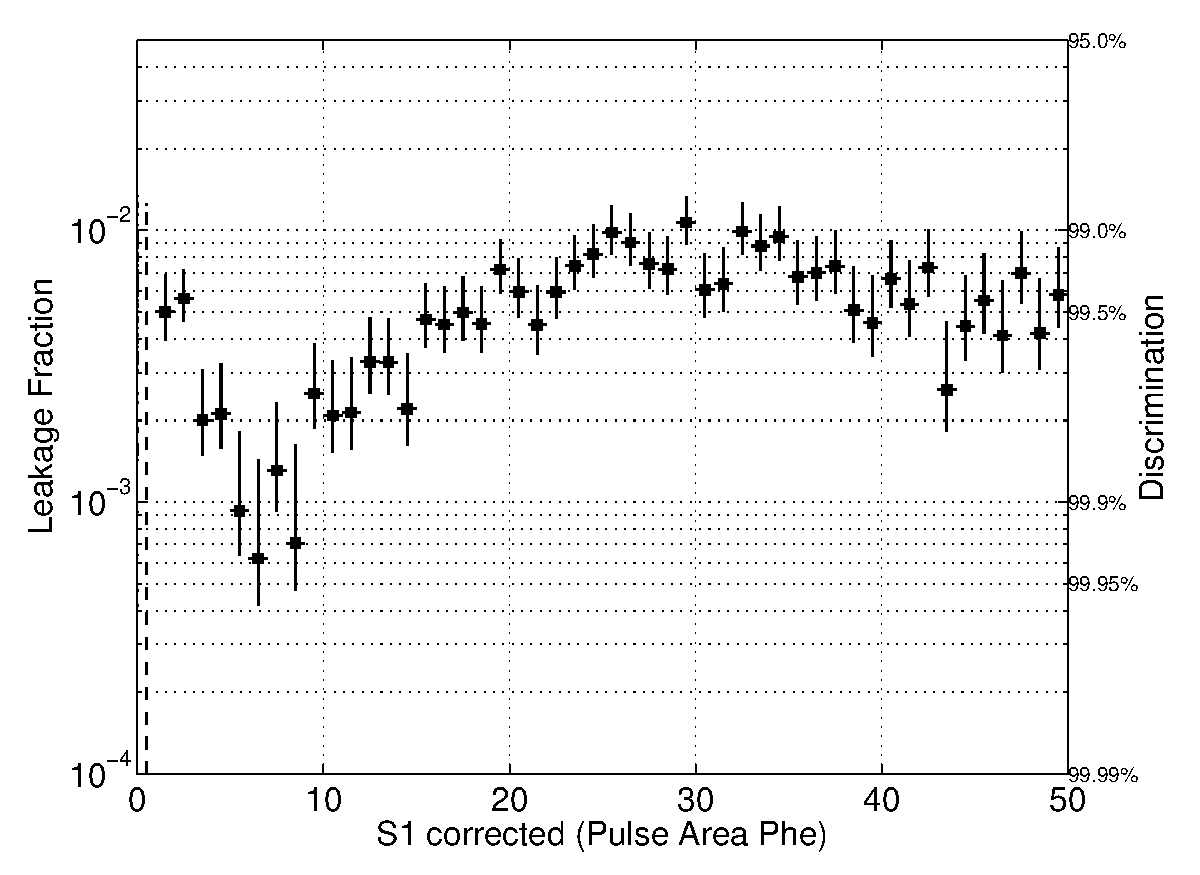
\includegraphics[width=80mm]{CH3T_Leakage_fid_50_Dec_Tritium_Approval_Plots.eps}
\caption{Discrimination vs. S1 using over 115,000 tritium beta decays between 1 and 50 Phe in S1 (about $\rm1-8 keV_{ee}$). On average from 1 to 30 Phe the discrimination is 99.58\%, defined by the fraction of events of events below the mean of the nuclear recoil band. The red band represents the NEST nuclear recoil band (version 4c) vetted with an AmBe, $\rm^{252}Cf$ and DD neutron generator calibration.}
\label{fig:Leak}
\end{figure}


%Figure \ref{fig:NEST_v_Data} shows the comparison between simulation(NEST) and the data for the ER band. The agreement between simulation and data is good down to 7 Phe in S1. This is expected since at sub 2 $\rm keV{ee}$ (7 Phe in S1) data is limited and the NEST model has yet to be vetted at such low energies[Matthew/ Erik Dahl Thesis]. The newly acquired ER data below 2 $\rm keV{ee}$ from tritium will be used improve upon the NEST model at the extration field of 180 V/cm [ref?].

\begin{comment}

\begin{figure}[h!]\centering
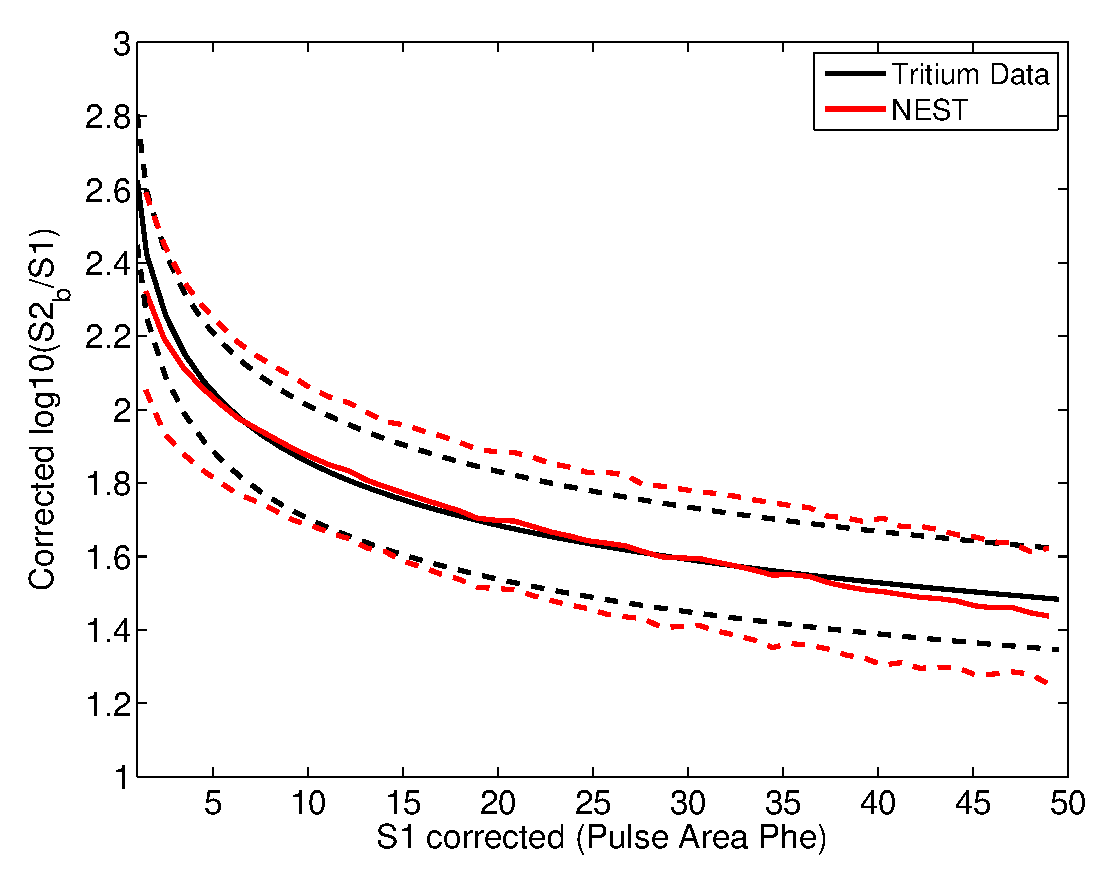
\includegraphics[width=80mm]{CH3T_DATA_NEST_fid_30_LUX_SIM_Tritium.eps}
\caption{ER band measured using tritium data in black with 90\% confidence bounds ( $\rm \pm 1.3 \sigma$) compared with the NEST prediction in red.}
\label{fig:NEST_v_Data}
\end{figure}
\end{comment}

%%%%%%%%%%%%%%%%%%%%%%%%%%%%%%%%%%%%%%%%%%%%%%%%%
\begin{comment}

\subsection{Threshold Determination}

The tritiated methane calibration source can also be used to determine detector efficiency for both S1 (primary scintillation) and S2 (secondary scintillation) down to sub 1 keV electronic recoils.The ultimate limitation of single scatter event is typically the S1 since the signal size of the S1 is one to three orders of magnitude less than the S2. We measured the threshold by comparing the NEST model of a tritium beta spectrum to the data, we find good agreement to the threshold determined from LED calibration, figure \ref{fig:S1S2_Thresh}(need to add to plot). The threshold for the S2 (bottom PMT array) shown is entirely due to the S1 threshold. We use only the bottom PMT array for the S2 signal because the secondary scintillation light is more uniformly distributed along the bottom PMTs than the top PMTs. Figure \ref{fig:E_spec} shows the tritium beta spectrum measured in the LUX detector along with the NEST prediction, note at the 180 V/cm drift field NEST has been vetted form 2 to 10 $\rm keV{ee}$.

\begin{figure}[h!]\centering
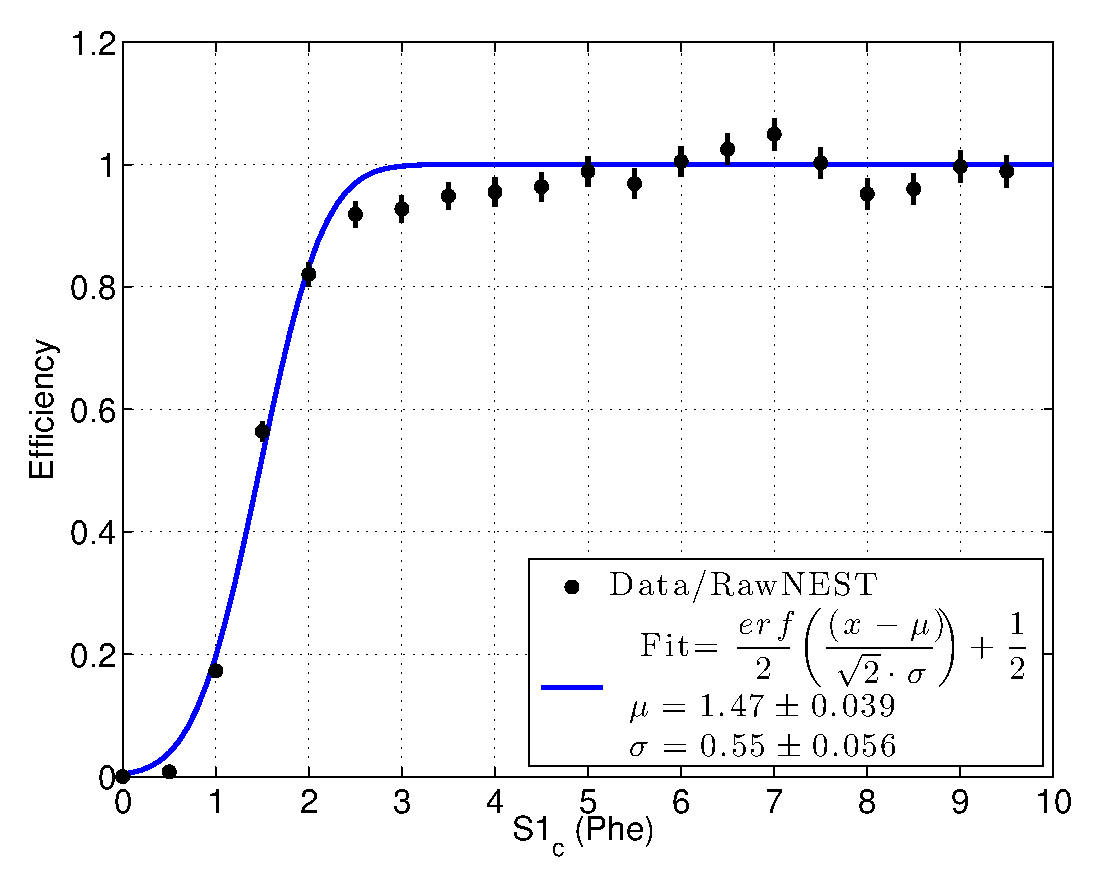
\includegraphics[width=80mm]{CH3T_eff_S1_100_T_paper_corr_threshold.eps}
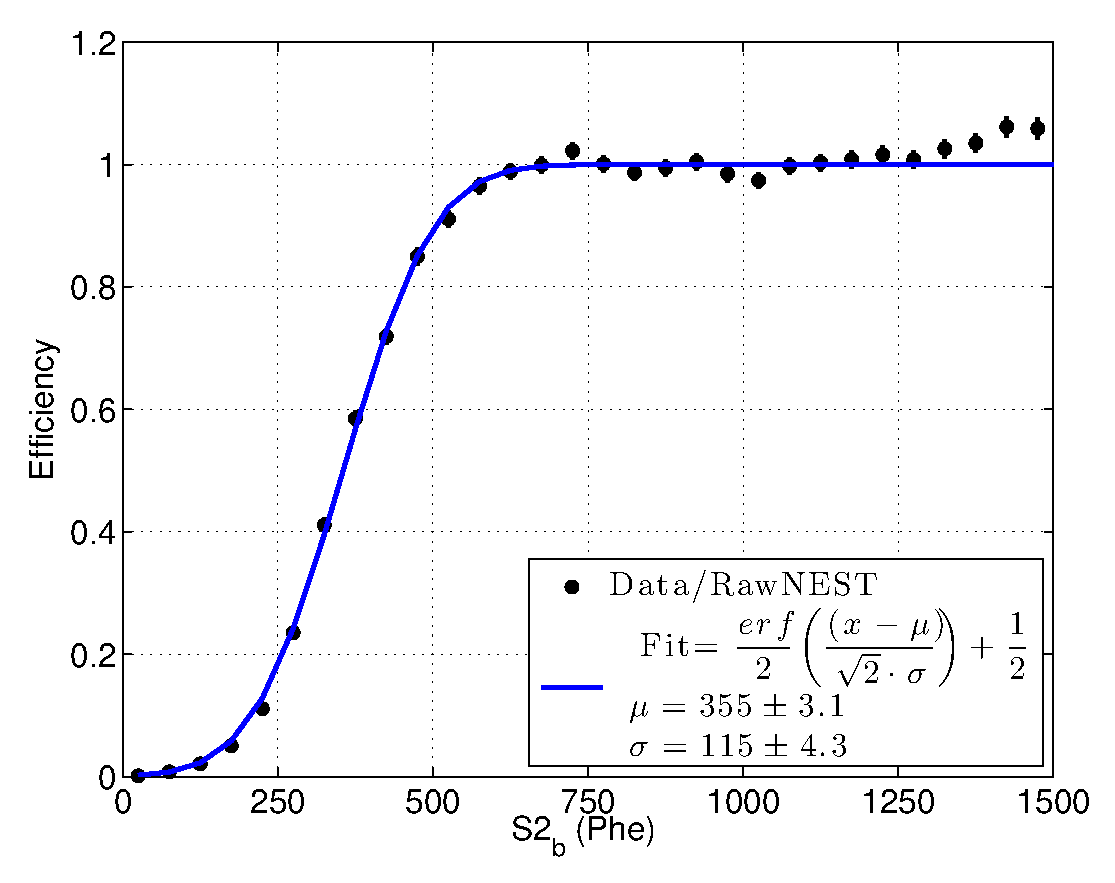
\includegraphics[width=80mm]{CH3T_eff_S2_100_T_paper_corr_threshold.eps}
\caption{S1 Threshold determined from Tritium. S2 Threshold determined from Tritium.}
\label{fig:S1S2_Thresh}
\end{figure}



\begin{figure}[h!]\centering
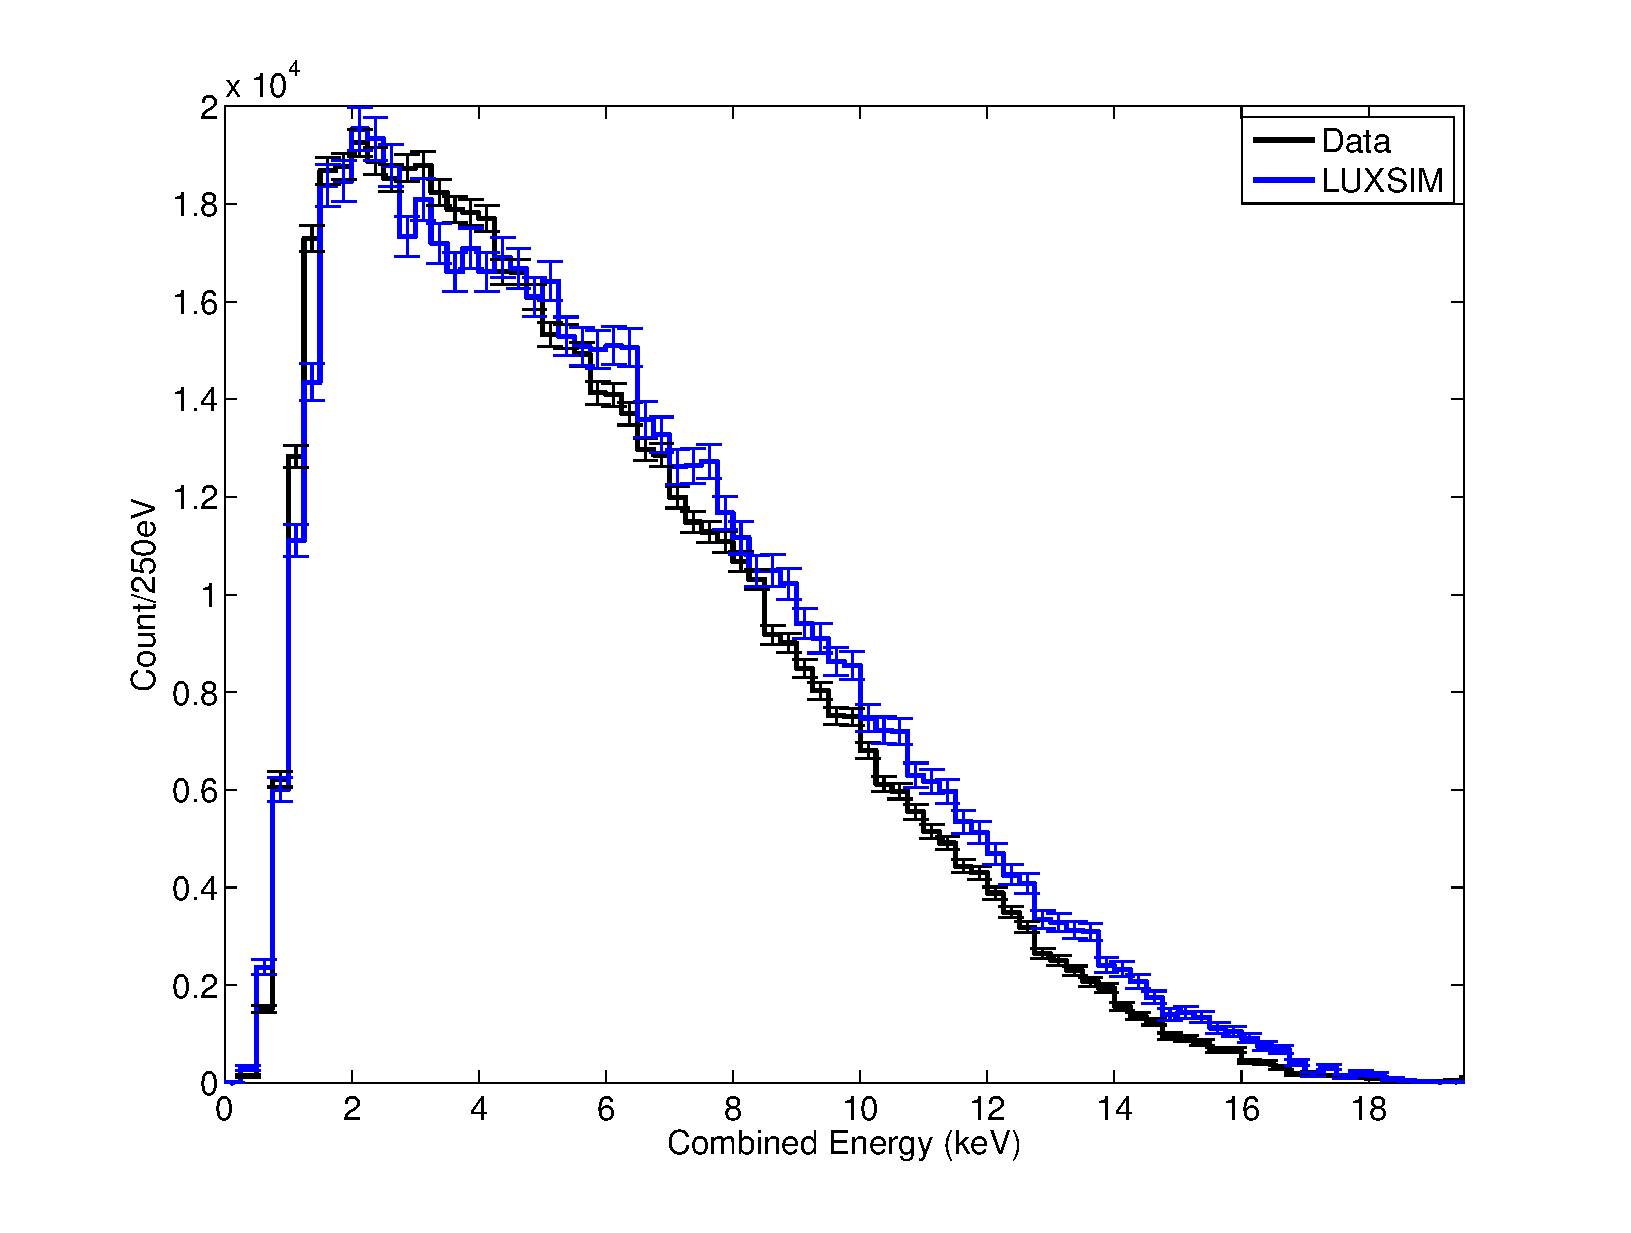
\includegraphics[width=80mm]{CH3T_E_spec_18_Tritium_Dec_2013_180.eps}
\caption{Combined energy spectrum of the tritium data and LUX SIM.}
\label{fig:E_spec}
\end{figure}
 


 
 \subsection{Absolute Rate}
The absolute efficiency for detecting tritium events can be determined by comparing the number of observed events to the number expected. The initial activity injected was calculated to be $0.84 \pm 0.22 $ Bq, with the largest uncertainty coming from the ratio of $\rm CH_3T/CH_4$ from the tritiated methane source bottle. The purification time constant was measured to be 6.6 hours. From the initial rate and the purification constant we expect to count a total of $20,200 \pm 4,000 $ events in the LUX detector before applying the S1 threshold. With the S1 threshold we expect  $16,000 \pm 3,100 $ `golden' events. The actual count observed in the liquid xenon volume was 20,000 events, which is in good agreement with the expected value taking into account the uncertainty in the initial activity and the purification model. After making fiducial cut $7,700 \pm  1,500$ events were expected and a total of $9,500 \pm 100$ were observed.
%,  roughly $16,000 \pm  3,100 * (290/324)*(18^2/24.5^2)$. 



\section{Scintillation Yield and Ionization Yield from Tritium Beta Decay}


\subsection{Cuts used in this analysis}
\begin{itemize}
\item Standard LUX Pulse finder classifier used in the WIMP search.
\item $\rm S2_b > 100 [Phe] $
\item PDE (g1) = 0.138 $\rm \pm 0.005$, measured with Tritium
\item Extraction = 0.664 $\rm \pm 0.04$ measured with Tritium.
\item single e- = 9.95 $\rm \pm 0.1$ [Phe/e-]
\item Using NEST 4c bands.
\end{itemize}




Scintillation and ionization yield are measured using the tritiated methane calibration source from the S1, S2 and reconstructed energy of each beta decay. The energy of each decay is determined using a prescription described in [Erik Dahl], see equations \ref{eq:Gain} and \ref{eq:E_comb}. 
\begin{equation}
\begin{split}
\rm  n_\gamma = \frac{S1}{g1}\\
\rm n_{e^{-}} = \frac{S2}{g2}
\label{eq:Gain}
\end{split}
\end{equation}

\begin{equation}
\begin{split}
\rm E= \frac{1}{W}(n_\gamma + n_{e^-})\\
\rm E= \frac{1}{W}(\frac{S1}{g1} + \frac{S2}{g2})
\label{eq:E_comb}
\end{split}
\end{equation}

The values of the work function W and gains g1, g2 have been measured using other calibration sources and are energy independent [ref]. Using equations \ref{eq:Gain} and \ref{eq:E_comb} we calculate the number of photons and electrons along with the energy of each tritium beta decay event to determine the yields. Scintillation and ionization yield are defined as [Photons/keV] and [Electrons/keV] respectively and the tritiated methane calibration source provides betas ranging from $\rm>1$ to 18 keV, with an exponential decline in event rate above 5 keV. For the results shown in figure \ref{fig:L_Q_Yield_180} over 150,000 beta decays in the fiducial volume were used to measure scintillation and ionization yield at 180 [V/cm]. A correction was applied for the beta spectral shape and the finite resolution of S1, S2 when measuring ionization and scintillation yield, the correction was found to be less than 10\% and is described in [my thesis]. Figure \ref{fig:L_Q_Yield_180} also shows the comparison of the results with the NEST model which has been vetted between 2 and 10 $\rm keV{ee}$. Also show are the measurements of light yield from a $\rm^{83m}Kr$ source, the 32.1 keV decay from $\rm^{83m}Kr$ is typically used as a standard calibration. (The second 9.4 keV decay from $\rm^{83m}Kr$  shown in the figure is for decays that occur more than 1000 ns after the initial 32.1 keV decay).

We find good agreement with the NEST model in the regions that have been vetted (2-10 $\rm keV{ee}$), see figure \ref{fig:L_Q_Yield_180}. Below 2 $\rm keV{ee}$ the light yield is lower than predicted by NEST and the charge yield is higher. The discrepancy between the data and the NEST model above 10 $\rm keV{ee}$ is due to limited data available for the model and also due to the track lengths of betas and gammas beginning to deviate above this energy. Note, under 10 $\rm keV{ee}$ track lengths of betas gammas are nearly identical. 

Figure \ref{fig:L_Q_Yield_Baudis} includes our light and charge yield measurements at 100 and 180 V/cm along with the recent Compton scattering measurement down to 1.5 $\rm keV{ee}$ from \cite{Baudis} at 450 V/cm. The error bars show in the figure include uncertainties from W, g1, g2 and the spectral shape correction. Unlike the measurement made using Compton scattering we can reconstruct energy using both the light and charge channels for each decay allowing for a powerful calibration down to 1 $\rm keV{ee}$ (corresponding to 80\% threshold at 2 Phe in S1).  We find a lower light yield than the centroids of the measurements in [ref Budias], however the the measurement is within reported errors. At our lower fields a higher light yield is expected than that measured at 450 V/cm due to less free charge separation.  The light yield of the 32.1 keV gamma from $\rm^{83m}Kr$ is shown on the figure as a measure of systematic uncertainty between the experiments. For the case of the standardized $\rm^{83m}Kr$ calibration source we find the expected behavior between the two experiments, a higher extraction field leads to lower light yield.

%\begin{figure}[h!]\centering
%\includegraphics[width=120mm]{LY_c_180_Tritium_Dec_2013_Charge_Yield_180_corr.png}
%\includegraphics[width=120mm]{CH3T_fid_E_S2_c_Tritium_Dec_2013_Charge_Yield_180_corr.png}
%\caption{Top: Scintillation yield vs. combined energy using tritium beta decay. Bottom: Ionization yield vs. combined energy using tritium beta decay. At a drift field of 180 [V/cm], in the fiducial volume, and containing over 150,000 beta decays. The endpoint of the tritium beta spectrum is 18.6 [keV]}
%\label{fig:L_Q_Yield}
%\end{figure}


 \begin{figure}[h!]\centering
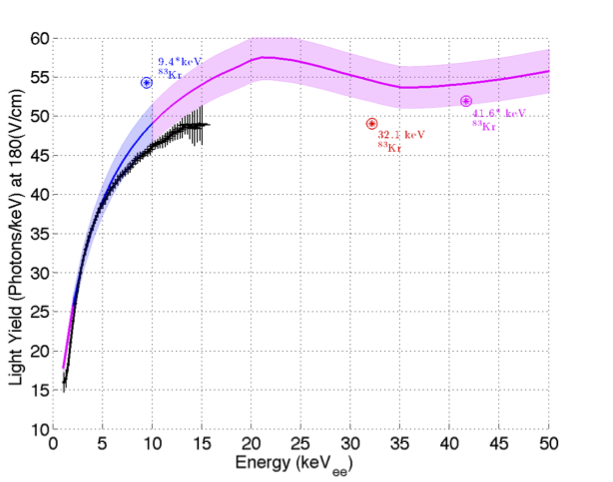
\includegraphics[width=80mm]{LY_180_band_Tritium_Dec_2013_Charge_Yield_180_corr.png}
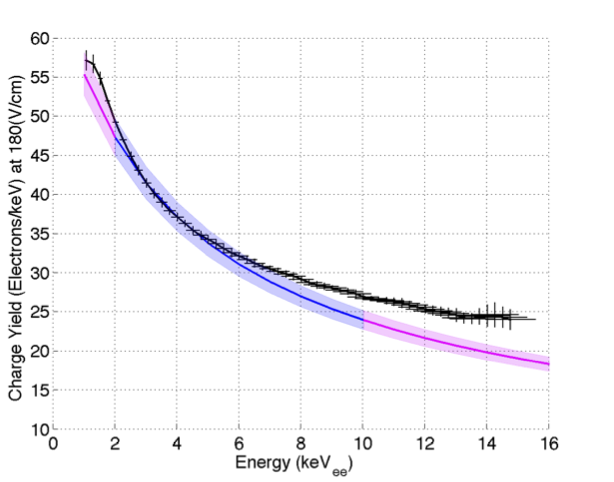
\includegraphics[width=80mm]{QY_180_Tritium_Dec_2013_Charge_Yield_180_corr.png}
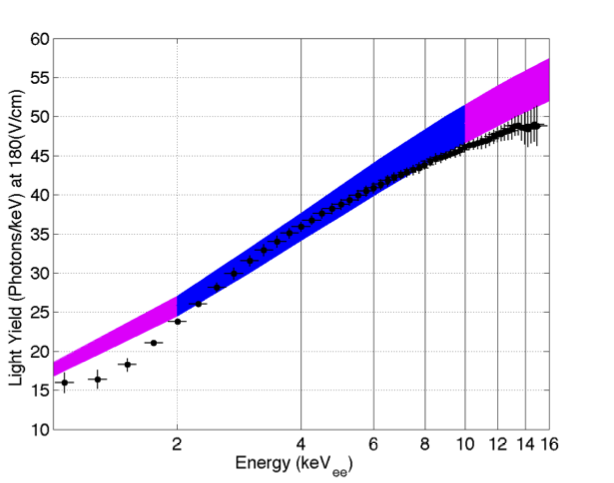
\includegraphics[width=80mm]{LY_180_band_log_Tritium_Dec_2013_Charge_Yield_180_corr.png}
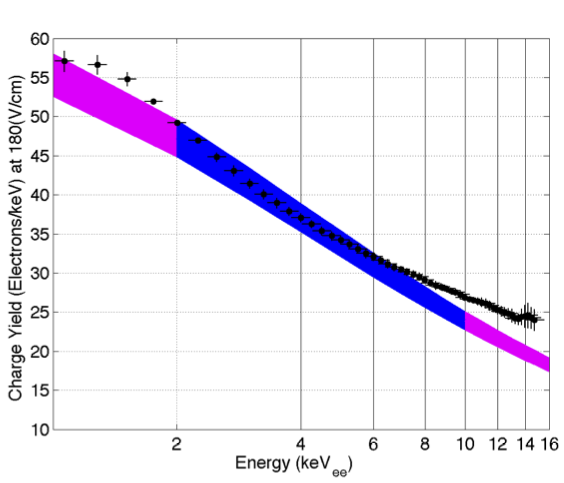
\includegraphics[width=76mm]{QY_180_log_Tritium_Dec_2013_Charge_Yield_180_corr.png}
\caption{180 [V/cm], corrected for spectral shape. Top Left: Mean scintillation yield vs. combined energy using tritium beta decay (black line). $\rm^{83}Kr$ lines are plotted for reference but only the 32.1 [keV] line (red star) is kosher since the 9.4 [keV] line is dependent on timing separation, the 9.4 [keV] line is plotted (blue star) for separations greater than 1000 [ns]. Top Right: Mean ionization yield vs. combined energy (black line). Bottom Left: Scintillation yield vs. combined energy on a log scale. Bottom Right: Ionization yield vs. combined energy on a log scale. The shaded blue regions represent the NEST mean with $\pm 5\%$ that has been vetted by data [Erik Dahl Thesis]. The shaded magenta regions represent the NEST extrapolations from data. The measurement is made at a field of 180 [V/cm] and contains over 150,000 beta decays. The endpoint of the tritium beta spectrum is 18.6 [keV]}
\label{fig:L_Q_Yield_180}
\end{figure}




 \begin{figure}[h!]\centering
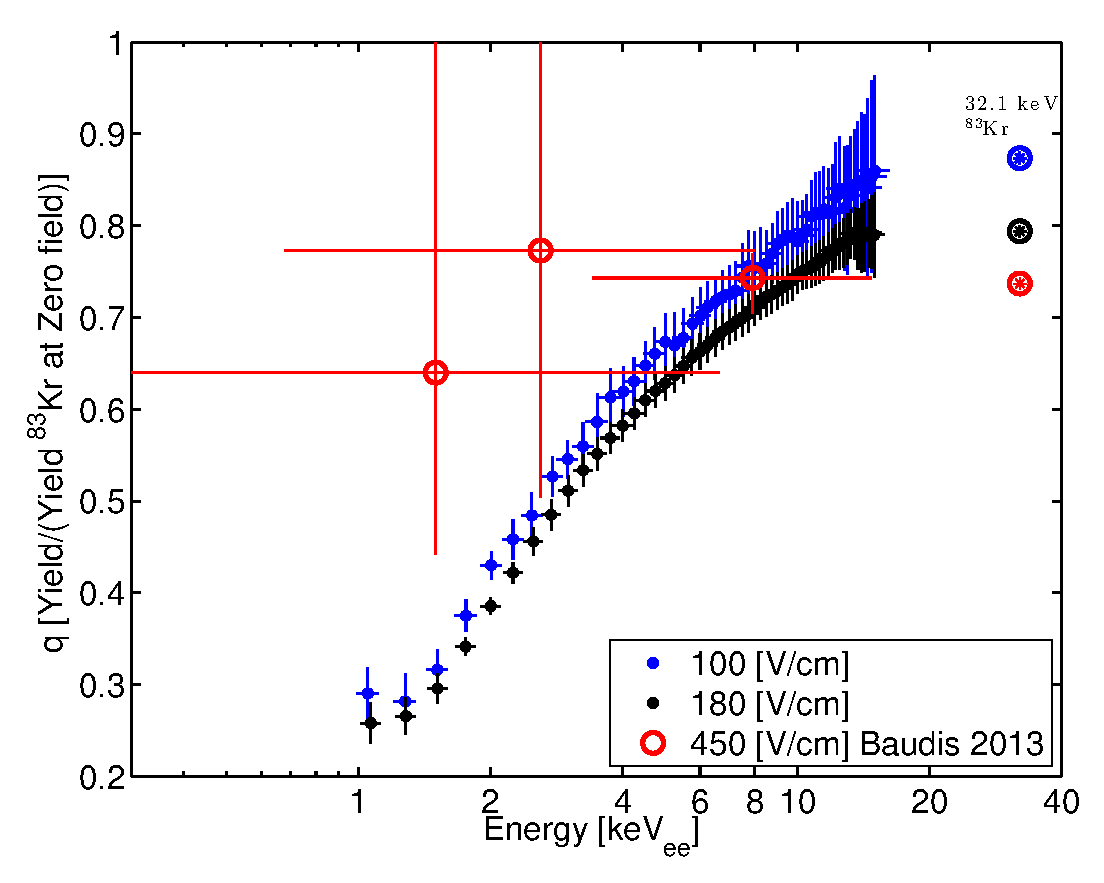
\includegraphics[width=80mm]{q_all_log_Tritium_Dec_2013_Charge_Yield_180_corr.eps}
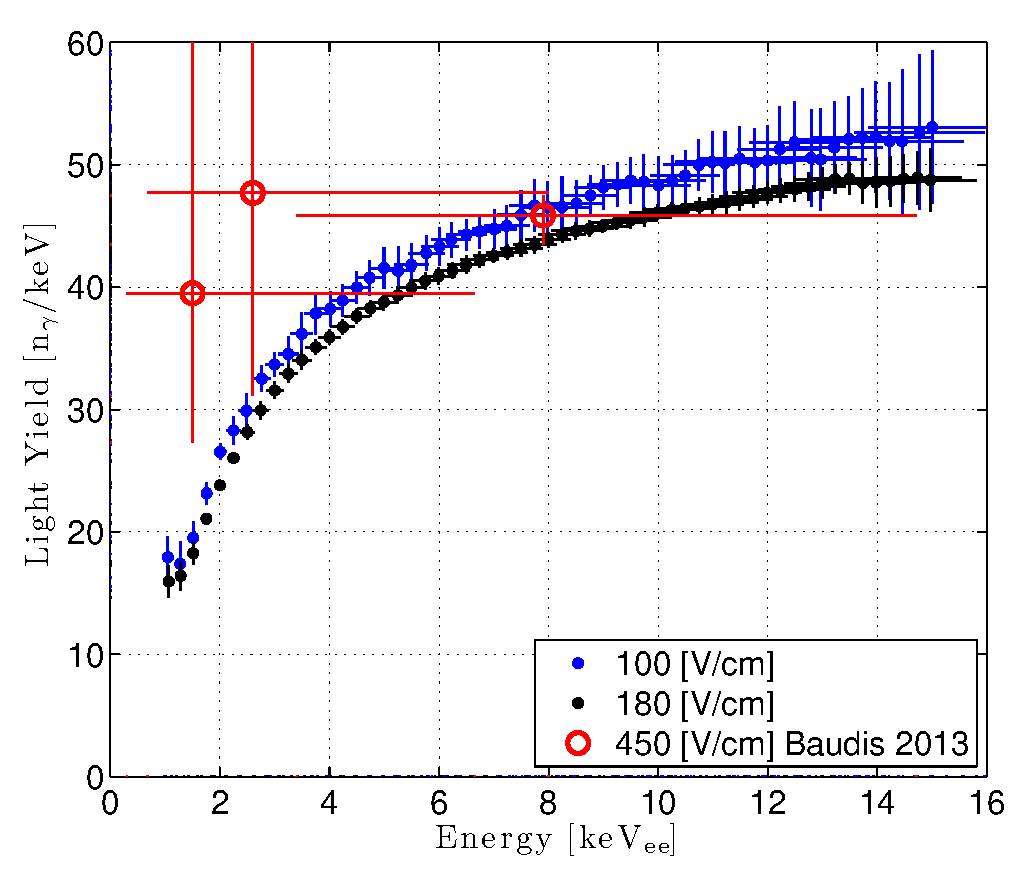
\includegraphics[width=80mm]{LY_all_Tritium_Dec_2013_Charge_Yield_180_corr.eps}
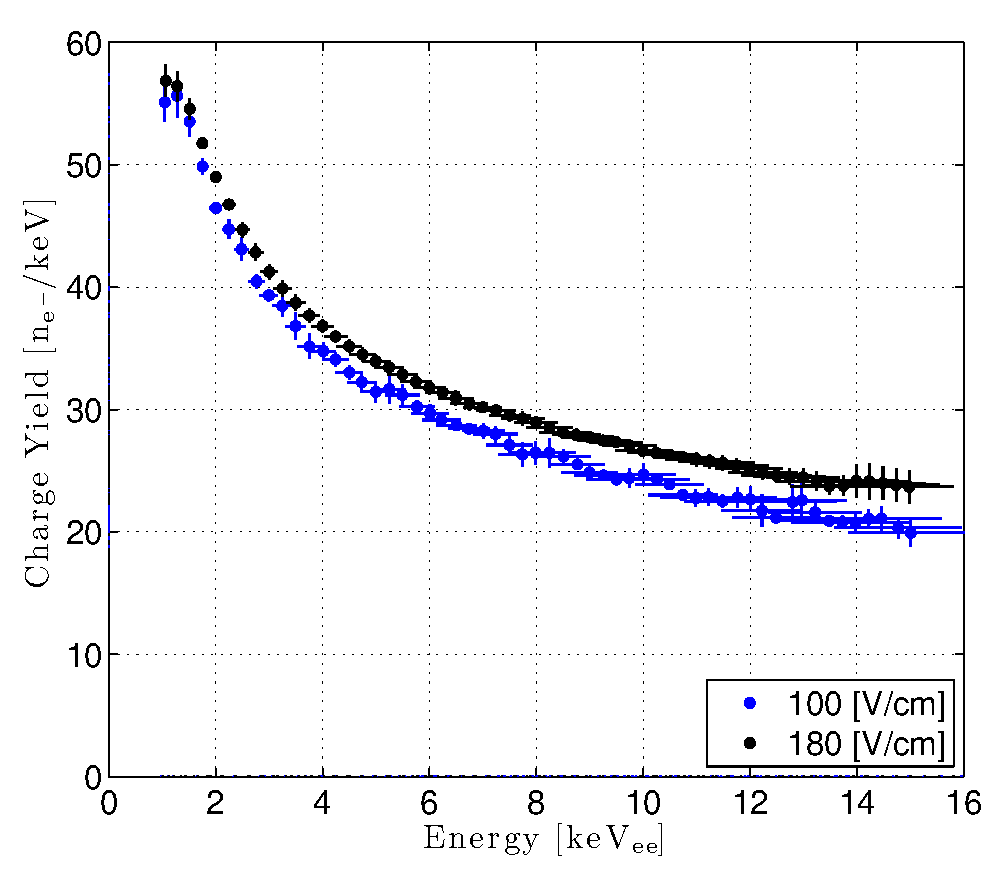
\includegraphics[width=80mm]{Charge_Y_all_Tritium_Dec_2013_Charge_Yield_180_corr.eps}
\caption{Top: Scintillation yield relative to the yield of the 32.1 gamma of [keV] $\rm^{83}Kr $  vs. Energy. Shaded blue curve is tritium at 100 [V/cm], shaded black curve is tritium at 180 [V/cm], red points represent a recent Compton scattering measurement at 450 [V/cm]. Also shown are the corresponding quenching of the 32.1 [keV]  gamma of $\rm^{83}Kr$ (star inside circle). Bottom: scintillation yield [Photons/keV] vs. Energy. Shaded blue curve is tritium at 100 [V/cm], shaded black curve is tritium at 180 [V/cm], red circles represent a recent Compton scattering measurement at 450 [V/cm].}
\label{fig:L_Q_Yield_Baudis}
\end{figure}



\end{comment}
%%%%%%%%%%%%%%%%%%%%%%%%%%%%%%%%%%%%%%%%%%%%%%%%%%%%%%%%%%

\section{All the things we can do with Tritium}

\begin{itemize}
\item Define the ER band.
\item Binned leakage fraction, and potentially optimize for spacial dependent leakage fraction in XYZ plane.
\item S1, S2 threshold. (Energy is a bit convoluted let's not go there). Requires NEST
\item Combined energy calibration to about 0.5 keVee. Requires NEST
\item Light Yield, Charge Yield. Requires some trivial smearing model, 10\% effect.
\item Fano-like factor vs. energy. Requires some trivial smearing model, sub 2\% effect.
\item Fiducial mass calculation, optimized for low energy S2s making it more WIMP like.
\item g1 and g2 calculation by competing tritium spectrum with NEST, or multiple E fields
\item ER band Gaussianity.
\item ... anything else?
\end{itemize}






\section{Summary}

We have characterized the electron recoil band and threshold of the LUX dark matter experiment with a tritium calibration source. The large dataset, high event purity, and simple topology provide a powerful tool to study the detector and to investigate the fundamental properties of LXe as a particle detection medium. The results presented here are used in an improved analysis of the Run 3 WIMP search data in Ref. \cite{lux-reanalysis}.


%\begin{acknowledgments}

%\end{acknowledgments}

%Use bibtex 

\bibliography{Tritium}{}
\bibliographystyle{plain}

%\bibitem{McKinsey} McKinsey, et al.  \emph{Journal of Physics: Conference Series} 203:012026 (2010) 
%\bibitem{Fiorucci} Fiorucci, et al.  \emph{AIP Conference Proceedings} 1200:977 (2010)
%\bibitem{Piche} R. Piche. \emph{Partial Differential Equations} Tampere University of Technology.
%\bibitem{Flanconneche} B. Flanconneche, J. Martin and M.H. Klopffer. "Permeability, Diffusion and Solubility of Gases in Polyethylene, Polyamide 11 and Poly(vinylidene fluoride)." \emph{Oil and Gas Technology}. Vol 1. 2001. p 261-278.


\end{document}

